\documentclass[12pt,onecolumn,a4paper,fleqn]{article}
\usepackage[top=1in, bottom=1in, left=0.75in, right=0.75in]{geometry}
\usepackage{epsfig,graphicx,amsthm,amsmath}
\usepackage[table,xcdraw,svgnames]{xcolor}
\usepackage{setspace}
\usepackage{mathtools}
\usepackage{fancyhdr}
\usepackage{sidecap}
\usepackage{caption}
\usepackage{subcaption}
\usepackage{hyperref}
\usepackage{tikz}
\usepackage{pgfplots}
\usetikzlibrary{decorations.pathreplacing}
\usepackage{relsize}
\usepackage{color,xcolor}
\usepackage[framed,numbered]{matlab-prettifier}
\usepackage{float}
\usepackage{enumerate}
\usepackage{booktabs}
\usepackage{wrapfig}
\usepackage{datetime}
\usepackage{xepersian}

\hypersetup{
	colorlinks=true,
	urlcolor=blue!70!black,
	linkcolor=blue
}


\settextfont[Path=fonts/,BoldFont={ZarBd.ttf},BoldFeatures={Scale=0.9}]{BZar.ttf}

%\DeclarePairedDelimiter\ceil{\lceil}{\rceil}
%\DeclarePairedDelimiter\floor{\lfloor}{\rfloor}

%\definecolor{vgreen}{RGB}{104,180,104}
%\definecolor{vblue}{RGB}{49,49,255}
%\definecolor{vorange}{RGB}{255,143,102}


% title page template
\newcommand{\heading}[2]
{
	\begin{center}
		{\huge
			\textbf{
				به نام خدا\\
			}
		}
		
		\vspace*{1.5cm}
		
\includegraphics[scale=0.9]{source/sharif_logo.png}\\
		\vspace*{0.5cm}
		{\Large
			\textbf{
				دانشگاه صنعتی شریف\\
				\vspace*{0.25cm}
				دانشکده مهندسی کامپیوتر\\
			}
		}
		\vspace*{3cm}
		{\huge
			\textbf{
				آزمایشگاه معماری کامپیوتر\\
				\vspace*{0.75cm}
			}
		}
		
		{\Large
			\textbf{
				#1:\\
				#2\\
			}
		}
		
		\noindent\rule[1ex]{\linewidth}{1pt}\\
		\vspace*{0.5cm}
		\begin{table}[H]
			\centering
			\begin{tabular}{|c|c|}
				\hline
				\multicolumn{2}{|c|}{\textbf{اطلاعات تیم}}
				\\ \hline
				\textbf{نام اعضا} & \textbf{شماره دانشجویی}
				\\ \hline
				متین داغیانی & 98106456
				\\ \hline
				بردیا محمدی & 98171104
				\\ \hline
				محمدجواد هزاره & 98101074
				\\ \hline 
			\end{tabular}
		\end{table}
		{\Large				
			\vspace*{0.75cm}
			\textbf{
				پاییز 1400
		}}		
	\end{center}
}

\pagestyle{fancy}
\fancyhf{}
\rhead{\textbf{آزمایشگاه معماری کامپیوتر}}
%%--------------------[should change]---------------------
\chead{\textbf{گزارش آزمایش چهارم}}
%%--------------------[should change]---------------------
\lhead{\textbf{\nouppercase{\rightmark}}}
\cfoot{({\thepage})}
\renewcommand{\headrulewidth}{1pt}
\renewcommand{\footrulewidth}{1pt}
\renewcommand{\sectionmark}[1]{\markright{#1}}
\renewcommand{\subsectionmark}[1]{\markright{#1}}
%\newdateformat{monthyeardate}{%
	%	\monthname[\THEMONTH], \THEYEAR}

\onehalfspacing
\begin{document}
	%%% title pages
	\large
	\begin{titlepage}
		\heading{آزمایش چهارم}{مبدل \lr{BCD} به باینری}
		\thispagestyle{empty}
	\end{titlepage}	
	\pagebreak
	
	%%% contents page
	\tableofcontents
	\thispagestyle{empty}
	\pagebreak
	
	%%% main document
	\section{هدف آزمایش}
	در این آزمایش هدف پیاده‌سازی مداری برای تبدیل اعداد ده‌دهی به باینری بود. عدد ورودی به صورت \lr{BCD} است و خروجی تبدیل شده‌ی این عدد در مبنای ۲ خواهد بود.
	
	به منظور تبدیل خواسته شده، از الگوریتم ارائه شده در گزارش‌کار استفاده شد که مراحل انجام آن به صورت مختصر در زیر آمده است:
	\begin{enumerate}
		\item
		عدد \lr{BCD} یک واحد به سمت راست شیفت داده شود.
		\item
		اگر بیت چهارم هر یک از ارقام ۱ است، آن رقم منهای ۳ شود.
		\item
		به مرحله ۱ رفته و مراحل تا جایی ادامه داده شود که تمام بیت‌های عدد \lr{BCD} برابر صفر شوند.
	\end{enumerate}
	در پایان این الگوریتم، بیت‌هایی که از سمت راست عدد خارج شده‌اند، نمایش باینری عدد مورد نظر را تشکیل خواهند داد.
	
	همانطور که از مراحل الگوریتم پیداست، برای طراحی مدار به یک تفریق‌کننده و رجیستر‌هایی برای نگه‌داری مقدار شیفت‌داده شده‌ی عدد ورودی نیاز است. به جای چک کردن صفر شدن تمام بیت‌ها، می‌توان از یک شمارنده استفاده کرد. در این آزمایش چون تعداد رقم‌های عدد ده‌دهی ورودی مشخص و برابر ۳ است، حداکثر مراحل الگوریتم برابر ۱۰ خواهد بود و درنتیجه می‌توان با شمارش تا ۱۰، به اتمام کار مدار پی برد. در ادامه به طراحی مدار داخلی ماژول‌های ذکر شده خواهیم پرداخت. نمای کلی مدار را نیز می‌توان در شکل \ref{fig:circuit} مشاهده کرد.
	\begin{figure}[H]
		\centering
		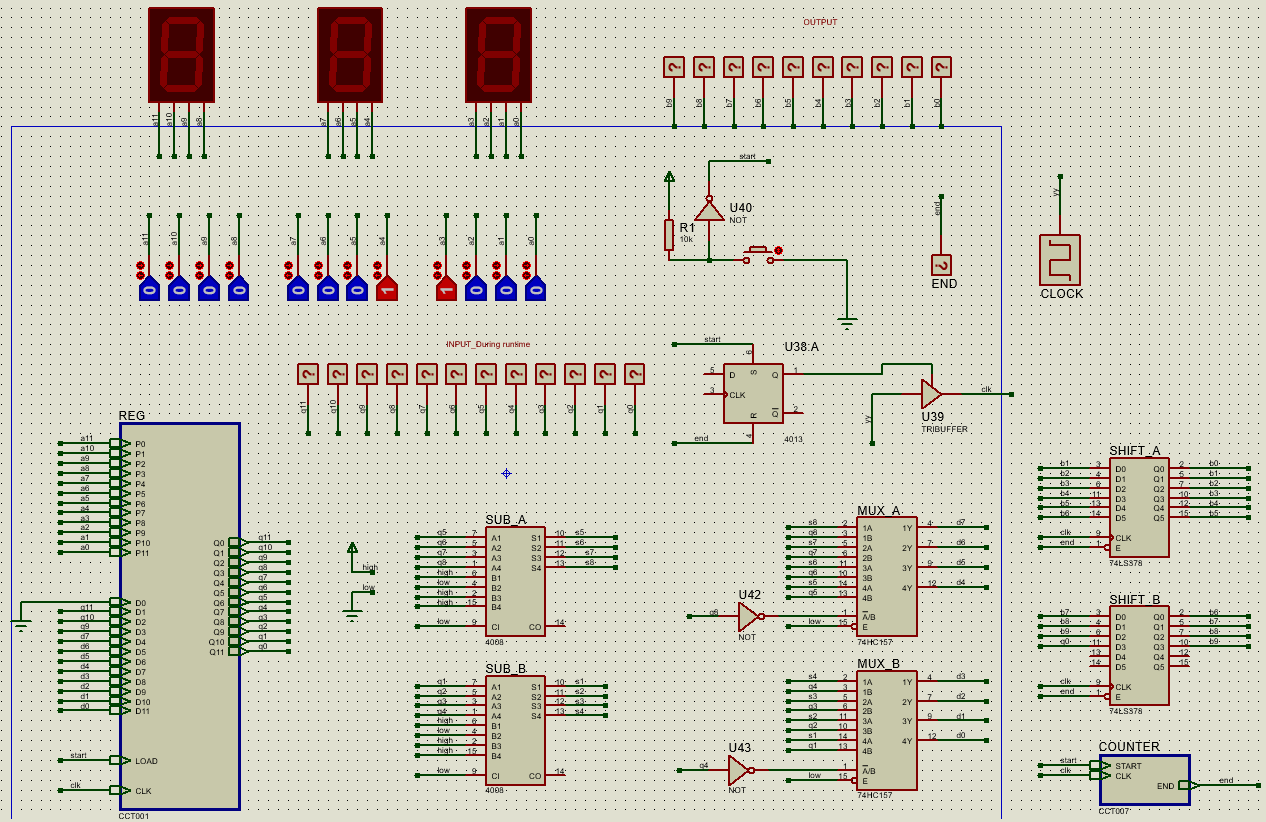
\includegraphics[width=0.8\textwidth]{source/circuit.png}
		\caption{نمای کلی مدار}
		\label{fig:circuit}
	\end{figure}
	\pagebreak
	\section{مراحل طراحی و پیاده‌سازی مدار}
	\subsection{ورودی و خروجی مدار}
	مطابق شکل \ref{fig:circuit} که در بخش قبل آمده است، ورودی مدار که عدد ده‌دهی مورد نظر است با بیت‌های $a_0$ تا
	$a_{11}$
	مشخص شده است و خروجی مدار که عدد دودویی 10 رقمی است با بیت‌های $b_0$ تا
	$b_{9}$.
	سیگنال‌های $q_0$ تا $q_{11}$ نیز همان عدد ده‌دهی ورودی را در طول مراحل الگوریتم نشان می‌دهند که به سمت راست شیفت داده می‌شود.
	
	سیگنال‌های $start$ و $end$‌ نیز به ترتیب برای فعال شدن مدار و مشخص کردن اتمام کار مدار استفاده می‌شوند. مطابق شکل \ref{fig:start-end}، برای سیگنال $start$ از یک پوش باتن استفاده شده که با فشردن این دکمه، فلیپ‌فلاپی که در تصویر وجود دارد ست شده و باعث فعال شدن کلاک مدار می‌شود. هم‌چنین با یک شدن سیگنال $end$، این فلیپ‌فلاپ ری‌ست شده و کلاک مدار از کار می‌افتد و کار آن به پایان می‌رسد.
	\begin{figure}[H]
		\centering
		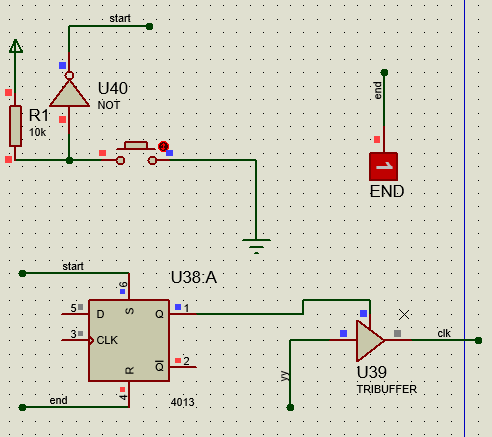
\includegraphics[width=0.5\textwidth]{source/start-end.png}
		\caption{عملکرد سیگنال‌های $start$ و $end$}
		\label{fig:start-end}
	\end{figure}
%	همانطور که در بخش قبل نیز بیان شد، ماژول‌های مدار شامل ماژول شیفت‌دهنده به راست، تفریق‌کننده و شمارنده می‌شوند. تعدادی ماژول مالتی‌پلکسر نیز برای تصمیم‌گیری نیاز است که در ادامه به بررسی طراحی داخلی تک تک این ماژول‌ها می‌پردازیم.
	\subsection{ماژول‌های \lr{SUB\_A} و \lr{SUB\_B}}
	\label{subsec:subtractor}
	وظیفه این ماژول کم کردن ۳ واحد از عدد داده شده به آن است. رابط آن را در شکل \ref{fig:sub} می‌توان دید و برای آن از ماژول‌های آماده‌ی پروتئوس استفاده شده است.
	\begin{figure}[H]
		\centering
		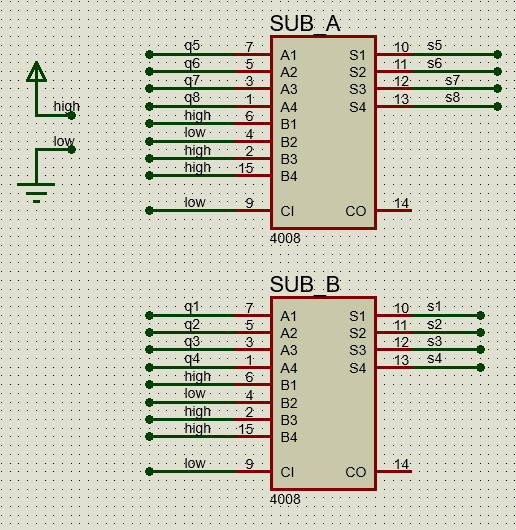
\includegraphics[width=0.5\textwidth]{source/sub.png}
		\caption{رابط ورودی و خروجی ماژول تفریق‌کننده}
		\label{fig:sub}
	\end{figure}
	با توجه به الگوریتم، اگر بیت باارزش هر یک از ارقام 1 باشد، باید سه واحد از آن کم کنیم. در این مدار چون ابعاد ورودی ثابت و برابر 3 رقم است، کافی‌ست فقط رقم‌های اول و دوم را بررسی کنیم؛ چرا که ابتدا شیفت به راست داده و سپس بیت باارزش را بررسی می‌کنیم، در نتیجه بیت باارزش رقم آخر همواره برابر صفر خواهد بود. به این منظور نخست رقم‌های اول و دوم را سه واحد کم کرده و سپس با استفاده از یک مالتی‌پلکسر و براساس بیت باارزش رقم مورد نظر تصمیم می‌گیریم از کدام عدد (عدد اولیه یا عددی که سه واحد از آن کم شده است) استفاده کنیم. همانطور که در شکل \ref{fig:sub} دیده می‌شود، ورودی دوم این ماژول متمم دو عدد ۳ است و ورودی اول آن در یک اینستنس از ماژول بیت‌های رقم اول و در دیگری بیت‌های رقم دوم است. خروجی آن نیز رقم اول منهای سه و رقم دوم منهای سه خواهد بود.
	\subsection{ماژول‌های \lr{MUX\_A} و \lr{MUX\_B}}
	\label{sec:mux}
	همانطور که در بخش
	(\nameref{subsec:subtractor})
	اشاره شد، نیاز داریم تصمیم بگیریم از بین رقم اولیه یا رقم منهای سه شده، یکی را انتخاب کنیم. این تصمیم براساس بیت باارزش آن رقم خواهد بود. وظیفه این ماژول‌ها انجام همین کار است. برای آن از ماژول‌های آماده‌ی پروتئوس استفاده شده است. ورودی و خروجی‌های آن‌ها را در شکل \ref{fig:mux} می‌توان دید.
	\begin{figure}[H]
		\centering
		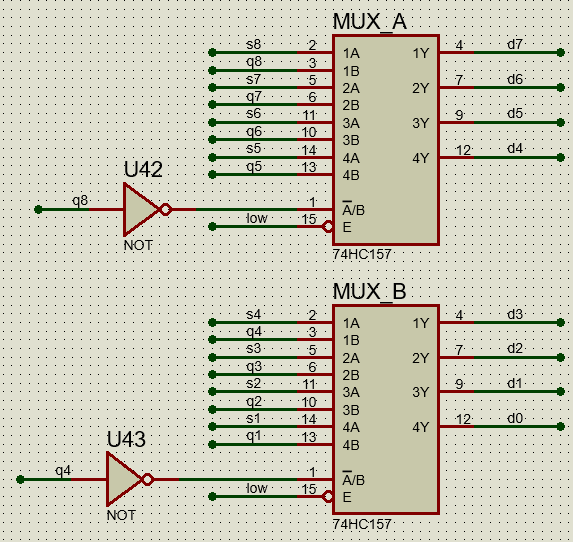
\includegraphics[width=0.5\textwidth]{source/mux.png}
		\caption{رابط ورودی و خروجی ماژول مالتی‌پلکسر}
		\label{fig:mux}
	\end{figure}
	همانطور که دیده می‌شود به ورودی‌های آن بیت‌های رقم اولیه ($q$ ها) و بیت‌های رقم منهای سه شده ($s$ ها) داده شده است. سلکتور آن نیز بیت باارزش رقم مورد نظر (در اینجا $q_4$) قرار داده شده است. (در اینستنس دیگر این ماژول، ‌سلکتور بیت باارزش رقم دوم یعنی $q_8$ قرار داده شده است.) هم‌چنین دقت کنید که از بیت‌های چهارم و هشتم استفاده شده، چرا که در مدار تفریق قبل از شیف‌دادن انجام و خروجی آن آماده شده است.
	\subsection{ماژول \lr{REG}}
	این ماژول وظیفه‌ی نگه‌داری مقدار ورودی را دارد. در مراحل مختلف الگوریتم نیاز به شیفت دادن ورودی به سمت راست داریم که مقدار آن پس از انجام شیفت در این ماژول ذخیره می‌شود. هم‌چنین این ماژول قابلیت بارگذاری موازی را نیز داراست، چرا که در ابتدای اجرای مدار نیاز داریم ورودی را در آن ذخیره کنیم. رابط این ماژول در شکل \ref{fig:reg} آمده است.
	\begin{figure}[H]
		\centering
		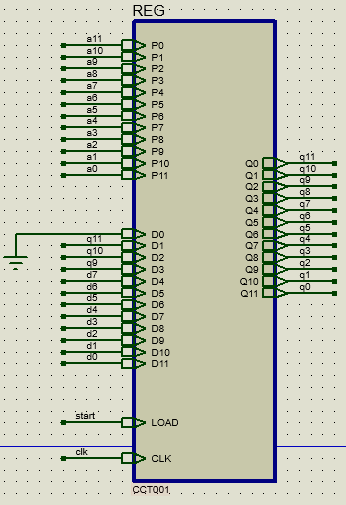
\includegraphics[width=0.5\textwidth]{source/reg.png}
		\caption{رابط ورودی و خروجی ماژول شیفت‌دهنده}
		\label{fig:reg}
	\end{figure}
	همانطور که در تصویر دیده می‌شود در ابتدا ورودی مدار یعنی سیگنال‌های $a_0$ تا $a_{11}$ در این ماژول بارگذاری می‌شوند. خروجی آن در هر لحظه سیگنال‌های $q_0$ تا $q_{11}$ خواهد بود که مقدار ورودی را در مراحل مختلف الگوریتم نشان می‌دهد. هم‌چنین ورودی‌های $D$ در این ماژول مقدار جدیدی هستند که قرار است در رجیسترها ذخیره شوند. این مقدار جدید از 12 بیت تشکیل شده که 4 بیت ابتدایی آن همان بیت‌های باارزش ورودی هستند که یک واحد به سمت راست شیفت داده شده‌اند. چهار بیت دوم، سیگنال‌های $d_4$ تا $d_7$ هستند که خروجی مالتی‌پلکسر \lr{MUX\_A} هستند. به همین ترتیب چهار بیت سوم، سیگنال‌های $d_0$ تا $d3$ هستند که خروجی مالتی‌پلکسر \lr{MUX\_B} می‌باشند. (برای مشخص شدن این که این سیگنال‌ها چه معنایی دارند به بخش (\nameref{sec:mux}) مراجعه کنید.) طراحی داخلی این ماژول را در شکل \ref{fig:reg-in} می‌توان مشاهده کرد.
	\begin{figure}[H]
		\centering
		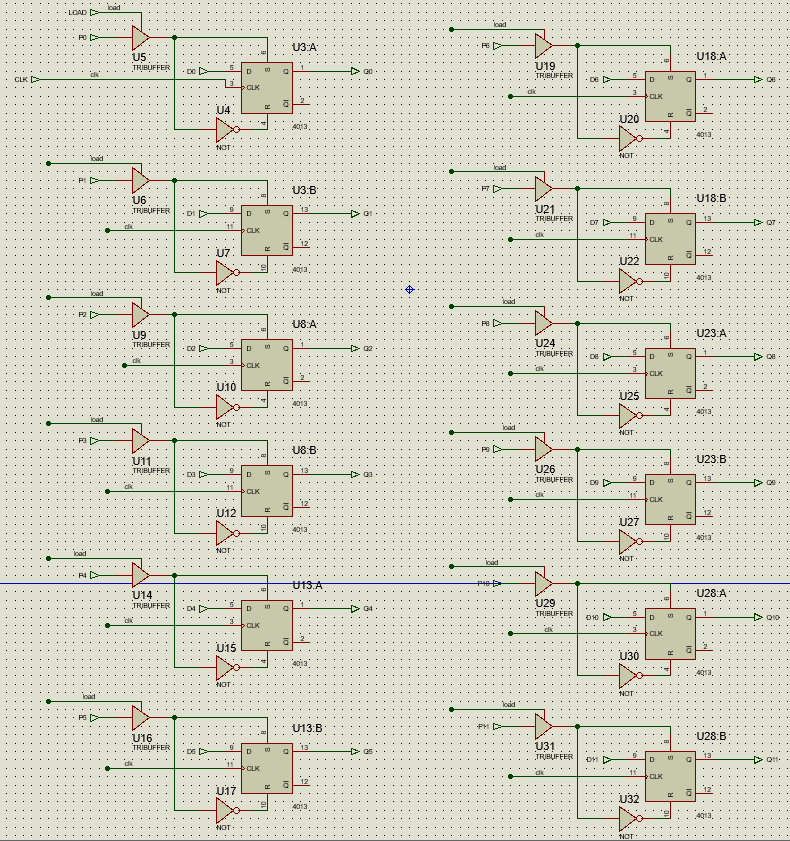
\includegraphics[width=0.8\textwidth]{source/reg-in.png}
		\caption{طراحی داخلی ماژول \lr{REG}}
		\label{fig:reg-in}
	\end{figure}
	همانطور که توضیح داده شد ورودی‌های $D$ به ورودی فلیپ‌فلاپ‌ها متصل شده و سیگنال‌ استارت فلیپ‌فلاپ‌ها به مقدار ورودی‌های $P$ با استفاده از یک ترای‌استیت بافر متصل شده است. این بافر زمانی فعال می‌شود که ورودی $Load$ ماژول فعال باشد.
	\subsection{ماژول‌های \lr{SHIFT\_A} و \lr{SHIFT\_B}}
	این ماژول‌ها وظیفه‌ی شیفت دادن به سمت راست خروجی را بر عهده دارند. ورودی و خروجی‌های آن‌ها در شکل زیر آمده است.
	\begin{figure}[H]
		\centering
		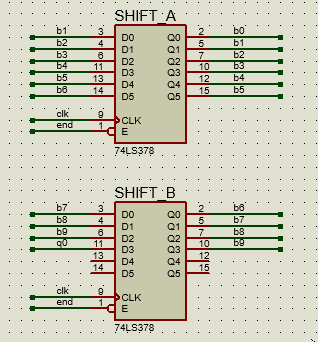
\includegraphics[width=0.5\textwidth]{source/shift.png}
		\caption{ورودی و خروجی ماژول‌های \lr{SHIFT\_A} و \lr{SHIFT\_B}}
		\label{fig:shift}
	\end{figure}
	برای این ماژول‌ها از ماژول‌های آماده‌ی پروتئوس استفاده شده است. همانطور که در تصویر دیده می‌شود ورودی $b_i$ به خروجی $b_{i-1}$ رفته و ورودی $q_0$ که همان بیت اول عدد ورودی‌ است، به خروجی $b_9$ می‌رود. با این‌کار در هر کلاک سیگنال‌های $b$‌ یک واحد به راست شیفت داده می‌شوند و بیت $q_0$ نیز از سمت چپ به آن‌ها اضافه می‌شود.
	\subsection{ماژول \lr{Counter}}
	وظیفه این ماژول شمارش تا عدد ۱۰ است. ورودی و خروجی‌های آن را در شکل \ref{fig:counter} می‌توان دید.
	\begin{figure}[H]
		\centering
		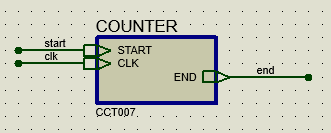
\includegraphics[width=0.4\textwidth]{source/counter.png}
		\caption{رابط ورودی و خروجی ماژول شمارنده}
		\label{fig:counter}
	\end{figure}
	همناطور که در تصویر دیده می‌شود، با آمدن سیگنال $start$ این ماژول شمارش خود را آغاز می‌کند و تا ۱۰ می‌شمارد و پس از اتمام شمارش سیگنال $end$ را فعال می‌کند. طراحی داخلی این ماژول را در شکل \ref{fig:counter-in} می‌توان مشاهده کرد.
	\begin{figure}[H]
		\centering
		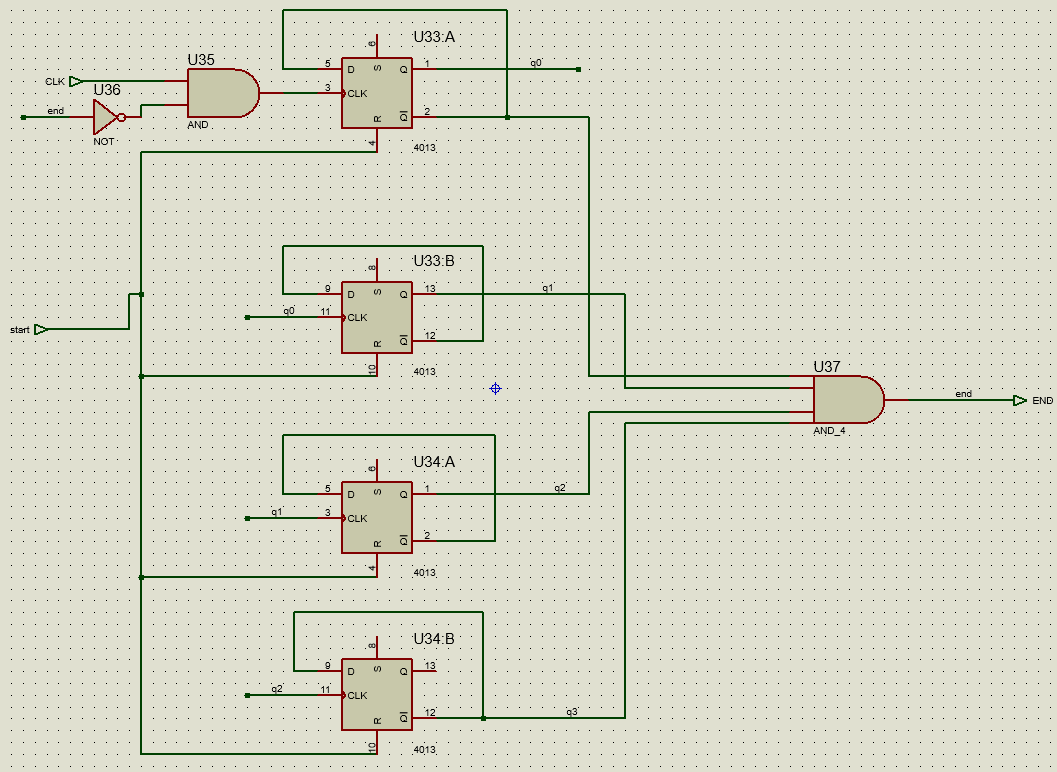
\includegraphics[width=0.7\textwidth]{source/counter-in.png}
		\caption{طراحی داخلی ماژول شمارنده}
		\label{fig:counter-in}
	\end{figure}
	\pagebreak
	\section{تست مدار}
	به منظور تست و شبیه‌سازی مدار، عملکرد مدار روی ورودی‌های مختلف بررسی شده است. در شکل‌هایی که در ادامه آمده است می‌توان خروجی و کارکرد مدار را به ازای ورودی‌های مختلف مشاهده کرد.
	\begin{figure}[H]
		\centering
		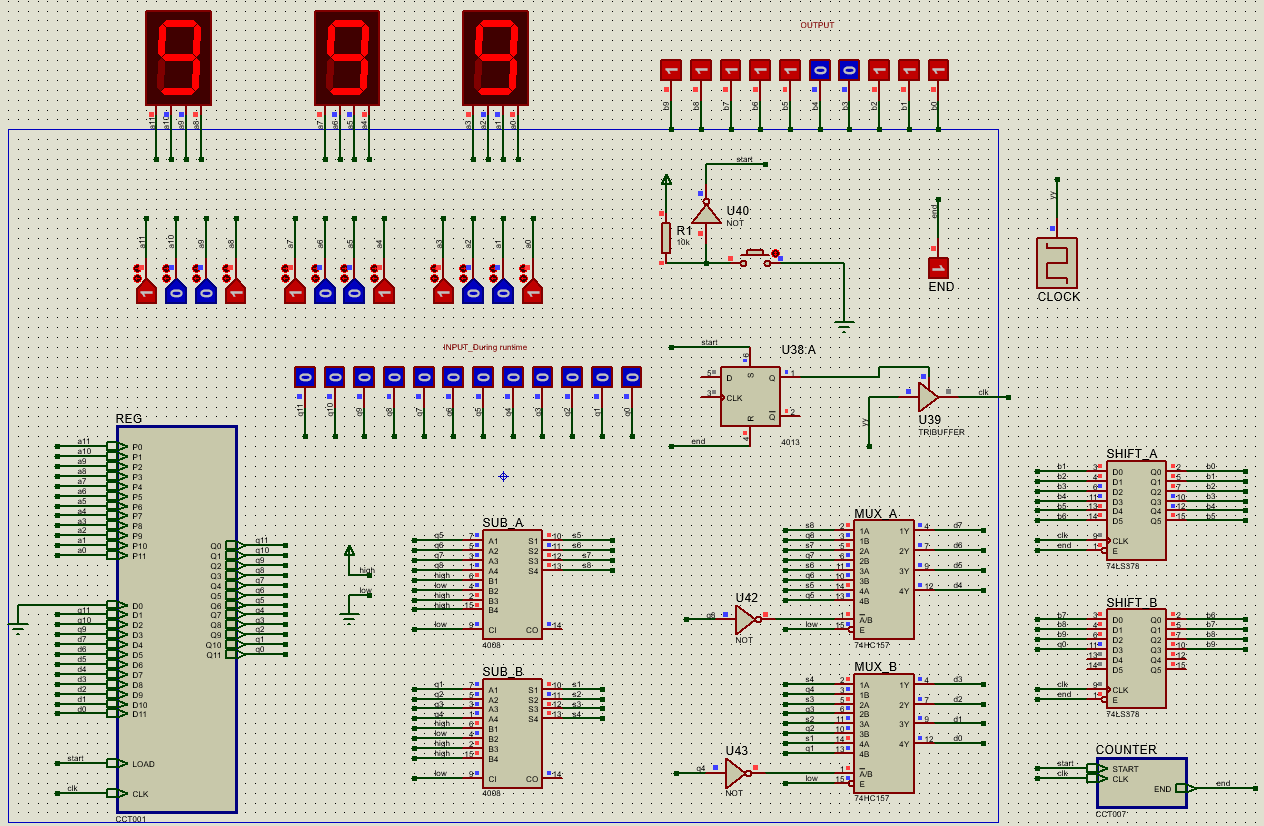
\includegraphics[width=0.8\textwidth]{source/test-999.png}
		\caption{تست مدار به‌ازای ورودی ۹۹۹}
	\end{figure}
	\begin{figure}[H]
		\centering
		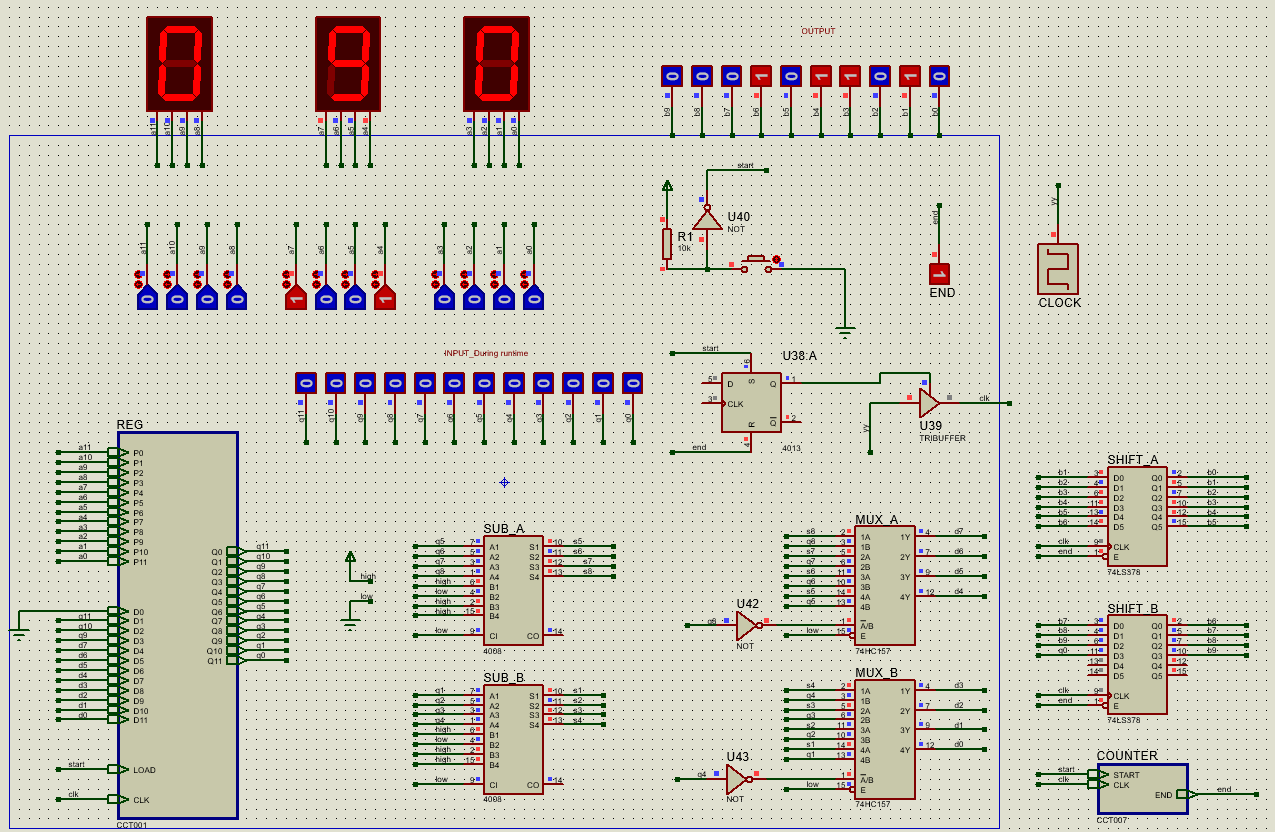
\includegraphics[width=0.8\textwidth]{source/test-90.png}
		\caption{تست مدار به‌ازای ورودی ۹۰}
	\end{figure}
	\begin{figure}[H]
		\centering
		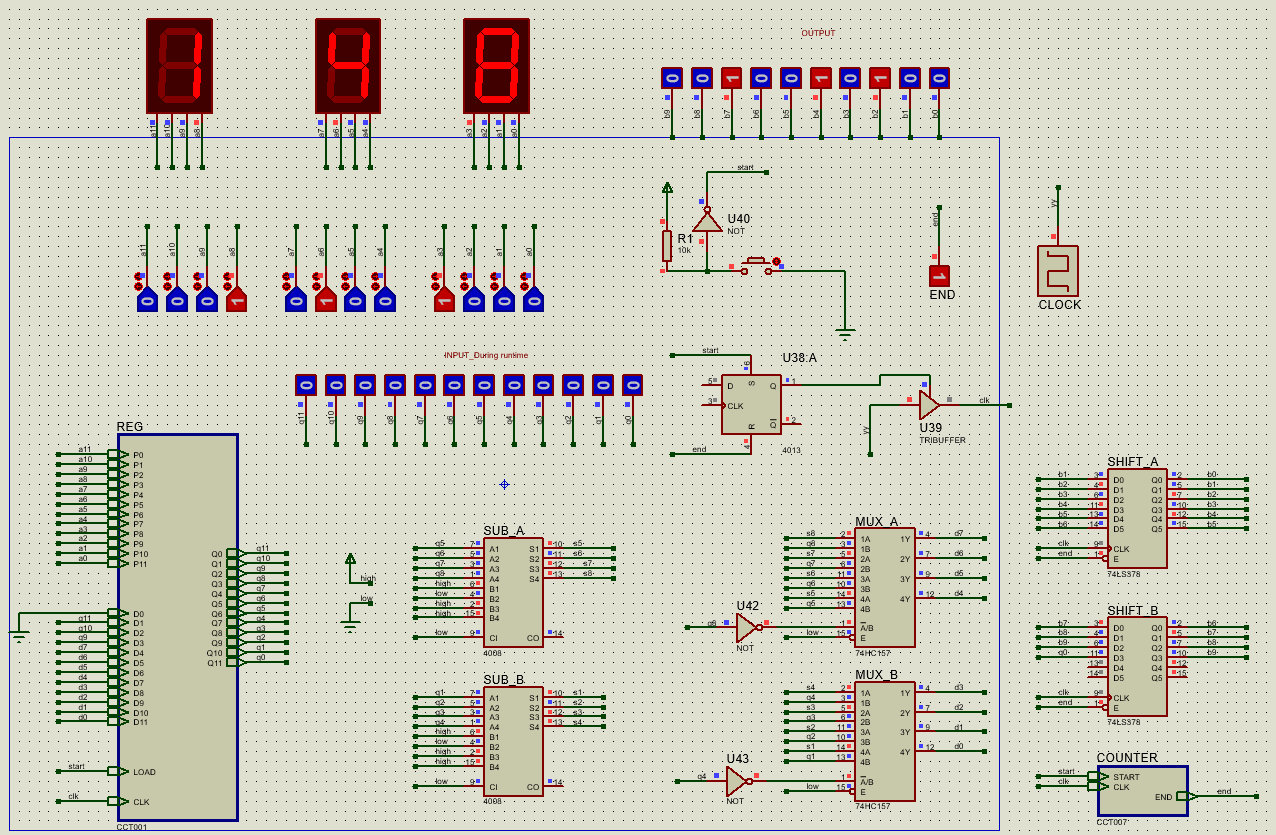
\includegraphics[width=0.8\textwidth]{source/test-148.png}
		\caption{تست مدار به‌ازای ورودی ۱۴۸}
	\end{figure}
	\begin{figure}[H]
		\centering
		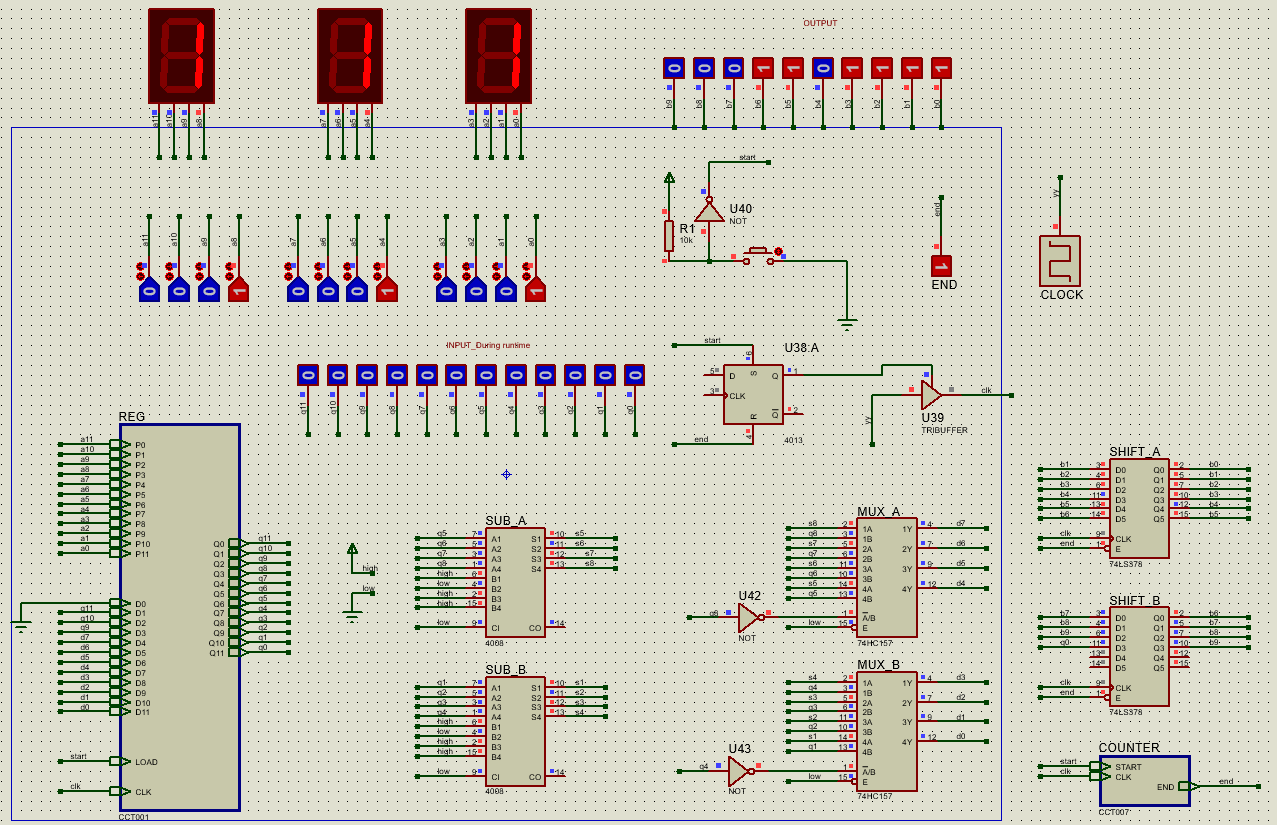
\includegraphics[width=0.8\textwidth]{source/test-111.png}
		\caption{تست مدار به‌ازای ورودی ۱۱۱}
	\end{figure}
\end{document}


